%%%%%%%%%%%%%%%%%%%%%%%%%%%%%%%%%%%%%%%%%%%%%%%%%%%%%%%%
%%%%%%%%%%%%%%%%%%%%%%%%%%%%%%%%%%%%%%%%%%%%%%%%%%%%%%%%
%%%%%%%%%%%%%%%%%%%%%%%%%%%%%%%%%%%%%%%%%%%%%%%%%%%%%%%%
%%%%%%%%%%%%%%%%%%%%%%%%%%%%%%%%%%%%%%%%%%%%%%%%%%%%%%%%
\documentclass[a4paper,12pt,twoside,openright]{report}
\usepackage[bibjustif]{abntex2cite}
\usepackage[brazil]{babel}
\usepackage{setspace}
\usepackage{amsthm}
\usepackage[figuresright]{rotating}
\usepackage{graphics}
\usepackage{amssymb}
\usepackage{graphicx}
\usepackage{fancybox}
\usepackage{amsmath}
\usepackage{picinpar}
\usepackage{colortbl}
\usepackage{wasysym}
\usepackage{txfonts}
\usepackage{pb-diagram}
\usepackage{relsize}
\usepackage{tikz}
\usepackage{pgfplots}
\usepackage{subfigure}
\usepackage{algorithm}
\usepackage{algorithmic}
\usepackage[hang,small,bf]{caption}
\usepackage[compact]{titlesec}
\usepackage[left=3cm,top=3cm,right=2cm,bottom=3cm]{geometry}%esq e sup 3cm  ; dir e inf 2cm
\usepackage[subfigure]{tocloft}
\usepackage{subfigure}

\renewcommand{\cftfigfont}{Figura }
\renewcommand{\cfttabfont}{Tabela }

\renewcommand{\cftfigaftersnum}{ - }
\renewcommand{\cfttabaftersnum}{ - }

\captionsetup{font=footnotesize,labelsep=endash}

\def\baselinestretch{1.6}
\pagestyle{myheadings}
\usepackage{enumitem}
\setlist[enumerate]{label*=\arabic*.}
\begin{document}
\titlespacing{\section}{0cm}{1.5cm}{1.5cm}
\titlespacing{\subsection}{0cm}{1.5cm}{1.5cm}

%%%%%%%%%%%%%%%%%%%%%%%%%%%%%%%%%%%%%%%%%%%%%%%%%%%%%%%%
%%%%%%%%%%%%%%%%%%%%%%%%%%%%%%%%%%%%%%%%%%%%%%%%%%%%%%%%
% CAPA
%%%%%%%%%%%%%%%%%%%%%%%%%%%%%%%%%%%%%%%%%%%%%%%%%%%%%%%%
%%%%%%%%%%%%%%%%%%%%%%%%%%%%%%%%%%%%%%%%%%%%%%%%%%%%%%%%
\setboolean{@twoside}{true}
\title{
	\vspace*{-120pt}
	\hspace*{+55pt}Universidade Estadual Paulista
	\newline
	\hspace*{+45pt}Instituto de Bioci\^{e}ncias, Letras e Ci\^{e}ncias Exatas
	\newline
	\hspace*{+30pt}Departamento de Ci\^{e}ncia da Computa\c{c}\~{a}o e Estat\'{i}stica
	\newline
	\newline
	\newline
	\hspace*{+50pt}Luis Fernando Teixeira Silva
	\newline
	\newline
	\newline
	Um sistema para reconhecimento de comandos falados dependente do locutor
}

\author{{\tiny .}}
\date{\vspace*{+60pt}S\~{a}o Jos\'{e} do Rio Preto - SP \\ 2017}
\maketitle

\newpage\
\thispagestyle{empty}

%%%%%%%%%%%%%%%%%%%%%%%%%%%%%%%%%%%%%%%%%%%%%%%%%%%%%%%%
%%%%%%%%%%%%%%%%%%%%%%%%%%%%%%%%%%%%%%%%%%%%%%%%%%%%%%%%
% PAGINA DE ROSTO
%%%%%%%%%%%%%%%%%%%%%%%%%%%%%%%%%%%%%%%%%%%%%%%%%%%%%%%%
%%%%%%%%%%%%%%%%%%%%%%%%%%%%%%%%%%%%%%%%%%%%%%%%%%%%%%%%
\pagestyle{empty}
\begin{tabular}{p{430pt}}
\pagestyle{empty}
\begin{center}
\pagestyle{empty}
\LARGE{\hspace*{+50pt}Luis Fernando Teixeira Silva\newline \newline \newline \newline \newline Um sistema para reconhecimento de comandos falados dependente do locutor}
\end{center}

\vspace*{+30pt}
\hspace*{+200pt}
\begin{tabular}{p{200pt}}
	\singlespacing{\small Monografia apresentada ao Programa de gradua\c{c}\~{a}o em Ci\^{e}ncia da Computa\c{c}\~{a}o da UNESP para obten\c{c}\~{a}o do t\'{i}tulo de Bacharel. \newline \newline Orientador: Prof. Dr. Rodrigo Capobianco Guido} \\
\end{tabular}
\newline 
\newline
\begin{center}
{\large S\~{a}o Jos\'{e} do Rio Preto - SP \\ 2017}
\end{center}
\end{tabular}

%%%%%%%%%%%%%%%%%%%%%%%%%%%%%%%%%%%%%%%%%%%%%%%%%%%%%%%%
%%%%%%%%%%%%%%%%%%%%%%%%%%%%%%%%%%%%%%%%%%%%%%%%%%%%%%%%
% FICHA CATALOGRAFICA
%%%%%%%%%%%%%%%%%%%%%%%%%%%%%%%%%%%%%%%%%%%%%%%%%%%%%%%%
%%%%%%%%%%%%%%%%%%%%%%%%%%%%%%%%%%%%%%%%%%%%%%%%%%%%%%%%


\begin{center}
	\vspace*{+260pt}
	{\footnotesize \hspace*{-81pt}Ficha catalogr\'{a}fica elaborada pelo Servi\c{c}o de Biblioteca do IBILCE/UNESP}
\end{center}

\vspace*{+5pt}

\begin{tabular}{|p{12.5cm}|}
	\hline
	{\singlespacing
		\vspace*{-20pt}
		\hspace*{+40pt} {\small Luis Fernando Teixeira Silva} \newline
		\hspace*{+40pt} {\small titulo} \newline
		\hspace*{+20pt} {\small titulo} \newline
		\hspace*{+20pt} {\small titulo. / fulano de tal; orientador} \newline
		\hspace*{+20pt} {\small Rodrigo Capobianco Guido. S\~{a}o Jos\'{e} do Rio Preto, 2017.} \newline
		\hspace*{+40pt} {\small xxx p.} \newline
		
		\hspace*{+40pt} {\small Monografia (TCC} \newline
		\hspace*{+20pt} {\small TCC} \newline
		\hspace*{+20pt} {\small TCC, 2017.} \newline \newline
		
		\hspace*{+40pt} {\small 1. Processamento de sinais. 2. Reconhecimento de locutor. 3. Ac\'{u}s-} \newline
		\hspace*{+20pt} {\small tica. 4. Energia. 5. Escala \textit{Bark}. I. Capobianco Guido, Rodrigo, orient.} \newline
		\hspace*{+20pt} {\small II. T\'{i}tulo.} \newline \newline
	}
	\\
	\hline
\end{tabular}

%%%%%%%%%%%%%%%%%%%%%%%%%%%%%%%%%%%%%%%%%%%%%%%%%%%%%%%%
%%%%%%%%%%%%%%%%%%%%%%%%%%%%%%%%%%%%%%%%%%%%%%%%%%%%%%%%
% FOLHA DE APROVACAO: MANTER EM BRANCO
%%%%%%%%%%%%%%%%%%%%%%%%%%%%%%%%%%%%%%%%%%%%%%%%%%%%%%%%
%%%%%%%%%%%%%%%%%%%%%%%%%%%%%%%%%%%%%%%%%%%%%%%%%%%%%%%%
\thispagestyle{empty}
\newpage\ \thispagestyle{empty} \newpage
\thispagestyle{empty}
\newpage\ \thispagestyle{empty} \newpage
\thispagestyle{empty}

%%%%%%%%%%%%%%%%%%%%%%%%%%%%%%%%%%%%%%%%%%%%%%%%%%%%%%%%
%%%%%%%%%%%%%%%%%%%%%%%%%%%%%%%%%%%%%%%%%%%%%%%%%%%%%%%%
% DEDICATORIA
%%%%%%%%%%%%%%%%%%%%%%%%%%%%%%%%%%%%%%%%%%%%%%%%%%%%%%%%
%%%%%%%%%%%%%%%%%%%%%%%%%%%%%%%%%%%%%%%%%%%%%%%%%%%%%%%%
\newpage
\thispagestyle{empty}
\vspace*{+480pt}
\hspace*{+160pt}
\begin{tabular}{p{200pt}}
	{\small Dedico este trabaho a todos os meus familiares, em especial aos meus pais, Nilda, Luis Carlos e a minha irm\~{a} Ana Beatriz.\newline Dedico tamb\'{e}m esse trabalho para a minha namorada Cristiana Luiza.}
\end{tabular}

\newpage\ \thispagestyle{empty} \newpage

%%%%%%%%%%%%%%%%%%%%%%%%%%%%%%%%%%%%%%%%%%%%%%%%%%%%%%%%
%%%%%%%%%%%%%%%%%%%%%%%%%%%%%%%%%%%%%%%%%%%%%%%%%%%%%%%%
% AGRADECIMENTOS
%%%%%%%%%%%%%%%%%%%%%%%%%%%%%%%%%%%%%%%%%%%%%%%%%%%%%%%%
%%%%%%%%%%%%%%%%%%%%%%%%%%%%%%%%%%%%%%%%%%%%%%%%%%%%%%%%
\newpage
\thispagestyle{empty}
\begin{center}{\LARGE \textbf{Agradecimentos}}\end{center}
\vspace{+60pt}
\par Primeiramente, gostaria de agradecer meus pais e minha madrinha, pois sem o apoio deles eu nunca teria conseguido ter acesso a um ensino de qualidade que o cursinho alternativo me proporcionou durante todo o ano de 2012. Foi gra{\c c}as a essas 3 pessoas que pude ingressar nessa linda universidade.

\par Gostaria de agradecer tamb\'{e}m a minha irm\~{a} que nos momentos mais dif\'{i}cies da minha gradua{\c c}\~{a}o me deu for{\c c}as para continuar em frente e concluir minha forma{\c c}\~{a}o de bacharel em ci\^{e}ncia da computa{\c c}\~{a}o. Agrade{\c c}o tamb\'{e}m a todos os meus familiares que me apoiaram ao longos dessa jornada de 5 anos.

\par E tamb\'{e}m deixo um agradecimento especial a meus dois grandes amigos Jo\~{a}o Cesar Granville e Luiz Gustavo Caobianco que tornaram esses anos na universidade mais felizes. Agrade{\c c}o tamb\'{e}m minha namorada por ter me auxilidado nesses dois \'{u}ltimos anos de universidade e por me dar for{\c c}as a concluir o curso nessa etapa final.

\newpage\ \thispagestyle{empty} \newpage

%%%%%%%%%%%%%%%%%%%%%%%%%%%%%%%%%%%%%%%%%%%%%%%%%%%%%%%%
%%%%%%%%%%%%%%%%%%%%%%%%%%%%%%%%%%%%%%%%%%%%%%%%%%%%%%%%
% PENSAMENTO
%%%%%%%%%%%%%%%%%%%%%%%%%%%%%%%%%%%%%%%%%%%%%%%%%%%%%%%%
%%%%%%%%%%%%%%%%%%%%%%%%%%%%%%%%%%%%%%%%%%%%%%%%%%%%%%%%
\newpage
\vspace*{+480pt}
\thispagestyle{empty}
\begin{flushright}
\textit{``No fim tudo d\'{a} certo, e se n\~{a}o deu certo \'{e} porque ainda n\~{a}o chegou ao fim.''}
\\
\textbf{Fernando Sabino}
\end{flushright}

\newpage\ \thispagestyle{empty} \newpage

%%%%%%%%%%%%%%%%%%%%%%%%%%%%%%%%%%%%%%%%%%%%%%%%%%%%%%%%
%%%%%%%%%%%%%%%%%%%%%%%%%%%%%%%%%%%%%%%%%%%%%%%%%%%%%%%%
% RESUMO E ABSTRACT
%%%%%%%%%%%%%%%%%%%%%%%%%%%%%%%%%%%%%%%%%%%%%%%%%%%%%%%%
%%%%%%%%%%%%%%%%%%%%%%%%%%%%%%%%%%%%%%%%%%%%%%%%%%%%%%%%
\newpage
\thispagestyle{empty}
\noindent
\begin{center}\textbf{\huge{Resumo}}\end{center} 
\vspace*{+60pt}
\begin{singlespace}
TAL, F. \textit{titulo}. 2016. xxxp. TCC UNESP 2016.
\end{singlespace}
\vspace*{+20pt}
Atualmente, ....
\\
\\
Palavras-chave: Processamento de sinais. Reconhecimento de locutor. Ac\'{u}stica. Escala \textit{Bark}.

\newpage\ \thispagestyle{empty} \newpage

\newpage
\thispagestyle{empty}
\noindent
\begin{center}\textbf{\huge{Abstract}}\end{center} 
\vspace*{+60pt}
\begin{singlespace}
TAL, F. \textit{titulo}. 2016. xxxp. TCC UNESP 2017.
\end{singlespace}
\vspace*{+20pt}
Nowadays, ...
\\
\\
Keywords: Signal processing. Speaker recognition. Acoustics. Bark scale.

\newpage\ \thispagestyle{empty} \newpage

%%%%%%%%%%%%%%%%%%%%%%%%%%%%%%%%%%%%%%%%%%%%%%%%%%%%%%%%
%%%%%%%%%%%%%%%%%%%%%%%%%%%%%%%%%%%%%%%%%%%%%%%%%%%%%%%%
% INDICES
%%%%%%%%%%%%%%%%%%%%%%%%%%%%%%%%%%%%%%%%%%%%%%%%%%%%%%%%
%%%%%%%%%%%%%%%%%%%%%%%%%%%%%%%%%%%%%%%%%%%%%%%%%%%%%%%%
%\pagestyle{empty}
\renewcommand
\listfigurename{\hspace*{+120pt} Lista de Figuras \thispagestyle{empty}}
\pagestyle{empty}
\listoffigures
%\pagestyle{empty}
\newpage\ \thispagestyle{empty} \newpage
%\pagestyle{empty}
\renewcommand
\listtablename{\hspace*{+120pt} Lista de Tabelas \thispagestyle{empty}}
%\pagestyle{empty}
\listoftables
%\pagestyle{empty}

\newpage\ \thispagestyle{empty} \newpage

%%%%%%%%%%%%%%%%%%%%%%%%%%%%%%%%%%%%%%%%%%%%%%%%%%%%%%%%
%%%%%%%%%%%%%%%%%%%%%%%%%%%%%%%%%%%%%%%%%%%%%%%%%%%%%%%%
% LISTA DE ABREVIACOES
%%%%%%%%%%%%%%%%%%%%%%%%%%%%%%%%%%%%%%%%%%%%%%%%%%%%%%%%
%%%%%%%%%%%%%%%%%%%%%%%%%%%%%%%%%%%%%%%%%%%%%%%%%%%%%%%%
\newpage
\thispagestyle{empty}
\vspace*{+62pt}
\begin{center}{\huge \textbf{Lista de Abreviaturas}}\end{center}
\vspace*{+20pt}
\begin{tabular}{l l}
\textbf{WAVE}&\textit{Waveform Audio File Format}
\\
\textbf{PCM}&\textit{Pulse-Code Modulation}
\\
\textbf{IBM}&\textit{International Business Machines}
\\
\textbf{RIFF}&\textit{Resource Interchange File Format}
\\
\textbf{fmt}&\textit{format}
\\
\textbf{IEEE}&\textit{Institute of Electrical and Eletronic Engineers}

\end{tabular}

%%%%%%%%%%%%%%%%%%%%%%%%%%%%%%%%%%%%%%%%%%%%%%%%%%%%%%%%
%%%%%%%%%%%%%%%%%%%%%%%%%%%%%%%%%%%%%%%%%%%%%%%%%%%%%%%%
% SUMARIO
%%%%%%%%%%%%%%%%%%%%%%%%%%%%%%%%%%%%%%%%%%%%%%%%%%%%%%%%
%%%%%%%%%%%%%%%%%%%%%%%%%%%%%%%%%%%%%%%%%%%%%%%%%%%%%%%%
\newpage\ \thispagestyle{empty} \newpage
%\pagestyle{empty}
\renewcommand
\contentsname{\hspace*{+160pt} Sum\'{a}rio \thispagestyle{empty}}
%\pagestyle{empty}
\tableofcontents
%\pagestyle{empty}

%%%%%%%%%%%%%%%%%%%%%%%%%%%%%%%%%%%%%%%%%%%%%%%%%%%%%%%%
%%%%%%%%%%%%%%%%%%%%%%%%%%%%%%%%%%%%%%%%%%%%%%%%%%%%%%%%
% CAPITULO 1
%%%%%%%%%%%%%%%%%%%%%%%%%%%%%%%%%%%%%%%%%%%%%%%%%%%%%%%%
%%%%%%%%%%%%%%%%%%%%%%%%%%%%%%%%%%%%%%%%%%%%%%%%%%%%%%%%
\setboolean{@twoside}{true}
\chapter{Introdu\c{c}\~{a}o}
\thispagestyle{myheadings}
\pagestyle{myheadings}
%%%%%%%%%%%%%%%%%%%%%%%%%%%%%%%%%%%%%%%%%%%%%%%%%%%%%%%%
% SECAO
%%%%%%%%%%%%%%%%%%%%%%%%%%%%%%%%%%%%%%%%%%%%%%%%%%%%%%%%
\section{Introdu\c{c}\~{a}o}
\label{cap1}
\par \textit{Speech recognition} ou reconhecimento de fala \'{e} uma \'{a}rea que ganhou destaque tanto no ambito cient\'{i}fico quanto no ind\'{u}strial. \'{E} comum encontrar nos \textit{shoppings}, \textit{smartphones}, \textit{notebooks} sistemas que fazem uso da computa{\c c}\~{a}o para poder realizar o reconhecimento de comandos, e essa realidade s\'{o} tende a aumentar com os avan{\c c}os da tecnologia em termos de \textit{hardware} e \textit{software}.

%%%%%%%%%%%%%%%%%%%%%%%%%%%%%%%%%%%%%%%%%%%%%%%%%%%%%%%%
% SECAO
%%%%%%%%%%%%%%%%%%%%%%%%%%%%%%%%%%%%%%%%%%%%%%%%%%%%%%%%
\section{Objetivo}
\par Este trabalho tem como objetivo implementar um algoritmo computacional desenvolvido em C/C++ para reconhecer comandos falados de modo \textit{off-line} com locutor pr\'{e}definido, ou seja \textit{speaker-dependent}. Esses comandos foram previamente gravados em arquivos no formato \textit{WAVE} de 16 \textit{bits} PCM.
%%%%%%%%%%%%%%%%%%%%%%%%%%%%%%%%%%%%%%%%%%%%%%%%%%%%%%%%

% SECAO
%%%%%%%%%%%%%%%%%%%%%%%%%%%%%%%%%%%%%%%%%%%%%%%%%%%%%%%%
\section{justificativa}
\par A \'{a}rea de \textit{speech recognition} nos \'{u}ltimos anos tem ganhado um grande destaque no ambito cient\'{i}fico, o que pode ser facilmente verificado atrav\'{e}s de consultas nos mais diversos reposi\'{o}rios digitais. Al\'{e}m disso, a \'{a}rea de estudo do presente trabalho tamb\'{e}m tem ganhado destaque na ind\'{u}stria com a populariza{\c c}\~{a}o dos \textit{smartphones} com reconhecimento de voz, o que justifica ainda mais a elabora{\c c}\~{a}o desse projeto.
\par Ademais, conv\'{e}m ressaltar que o presente trabalho utiliza a computa{\c c}\~{a}o junto com f\'{o}rmulas matem\'{a}ticas como parte de um ferramental para a resolu{\c c}\~{a}o de um problema da \'{a}rea de \textit{speech recognition}. 
%%%%%%%%%%%%%%%%%%%%%%%%%%%%%%%%%%%%%%%%%%%%%%%%%%%%%%%%

% SECAO
%%%%%%%%%%%%%%%%%%%%%%%%%%%%%%%%%%%%%%%%%%%%%%%%%%%%%%%%
\section{Motiva\c{c}\~{a}o}
\par Em 2008, \'{e} lan{\c c}ado o primeiro filme do Homem de Ferro, centrado no personagem Tony Stark. O filme al\'{e}m de despertar o interesse nas hist\'{o}rias em quadrinhos da Marvel, tamb\'{e}m prende a aten{\c c}\~{a}o dos ci\^{e}ntistas da computa{\c c}\~{a}o, uma vez que o personagem principal interage com uma intelig\^{e}ncia artificial - Jarvis - que podia controlar a casa e a armadura do h\'{e}roi. Vale ressaltar que Jarvis al\'{e}m de fazer reconhecimento do locutor de modo \textit{speaker-dependent}, tamb\'{e}m realizada s\'{i}ntese de voz. J\'{a} no ano de 2011, foi lan{\c c}ado a primeira vers\'{a}o do assistente pessoal do iOS, conhecido como Siri, que permite que o usu\'{a}rio execute determinadas fun{\c c}\~{o}es do \textit{smartphone} utilizando comandos falados. E mais recente, o criador do Facebook, decidiu no ano 2016, implementar seu pr\'{o}prio assistente pessoal, que funciona tamb\'{e}m de modo dependente do locutor, para auxiliar nas tarefas dom\'{e}sticas.
\par FALAR SOBRE ALGUM CONTEXTO CIENTIFICO TAMBEM.
\par E \'{e} a partir desse contexto que surgiu a inspira{\c c}\~{a}o para o desenvolvimento desse trabalho. Inicialmente, o projeto tinha como proposta de conseguir auxiliar em determinadas fun{\c c}\~{o}es de uma resid\^{e}ncia, al\'{e}m de executar comandos b\'{a}sico em um computador. Por\'{e}m, o projeto necessitou de cortes em seu escopo para que se tornasse fact\'{i}vel sua elabora{\c c}\~{a}o como forma de trabalho de conclus\~{a}o de curso.
\par Assim, este projeto tem como objetivo iniciar o desenvolvimento de um futuro assitente pessoal, atrav\'{e}s da elabora{\c c}\~{a}o de um sistema para reconhecimento de comandos falados \textit{speaker-dependent}. 
%%%%%%%%%%%%%%%%%%%%%%%%%%%%%%%%%%%%%%%%%%%%%%%%%%%%%%%%

% SECAO
%%%%%%%%%%%%%%%%%%%%%%%%%%%%%%%%%%%%%%%%%%%%%%%%%%%%%%%%
\section{Metodologia}
\par Para a elabora\c{c}\~{a}o deste projeto foi determinado os seguintes 11 comandos:
\begin{itemize}
	\item{}Bom dia, Logan;
	\item{}Bom noite, Logan;
	\item{}Oi, Logan;
	\item{}Como est\'{a} o tempo hoje?;
	\item{}vai chover?;
	\item{}Abrir calculadora;
	\item{}Ver not\'{i}cias;
	\item{}Pesquisar;
	\item{}Alarme;
	\item{}Calend\'{a}rio;
	\item{}Sair;	
\end{itemize}
sendo que posteriormente foi realizada a grava\c{c}\~{a}o de 10 \'{a}udios para cada um dos 11 comandos referidos, totalizando 110 arquivos de \'{a}udio no formato MPEG-4.Tais arquivos foram convertidos para o formato \textit{WAVE} de 16 \textit{bits} PCM usando o programa \textit{Audacity}. Vale ressaltar que todos os \'{a}udios foram gravados em um ambiente que proporciona-se um certo grau de isolamento sonoro, para assim se obter um som com menos ru\'{i}do.
\par A partir dessa etapa inicial foi feita a extra\c{c}\~{a}o dos dados brutos contidos nos arquivos \textit{WAVE}. Para isso foi utilizada uma biblioteca fornecida pelo Prof.Dr.Rodrigo Capobianco Guido do Departamento de Ci\^{e}ncia da Comput{\c c}\~{a}o e Estat\'{i}stica (DCCE), IBILCE/Unesp. Tal biblioteca, escrita em C/C++, tem a fun\c{c}\~{a}o de separar o cabe{\c c}alho dos arquivos \textit{WAVE}. A partir desse ponto, a biblioteca foi modificada para extrair os dados brutos e guardar as amplitudes dos sinais em arquivos de texto. Foi realizada a automa{\c c}\~{a}o de todo o processo que exigia interven{\c c}\~{a}o humana para a execu{\c c}\~{a}o do algoritmo, como a passagem  de \'{a}udios como par\~{a}metro a cada nova execu{\c c}\~{a}o, cria{\c c}\~{a}o de arquivos para extra{\c c}\~{a}o dos valores das amplitudes dos sinais, entre outros. Toda essa automatiza{\c c}\~{a}o foi implementada com a utiliza{\c c}\~{a}o de \textit{scripts} escritos na linguagem \textit{Shell script}.
\par Posteriormente a etapa de extra{\c c}\~{a}o das amplitudes dos sinais digitalizados, foi realizada a extra{\c c}\~{a}o das caracter\'{i}sticas dos \'{a}udios analisados. Essa etapa consiste na utiliza{\c c}\~{a}o do m\'{e}todo A3 - descrito com maiores detalhes no cap\'{i}tulo \ref{cap2} - para obter assim, vetores de caracter\'{i}sticas. Tal processo \'{e} essencial no presente trabalho, pois os valores obtidos no processo de extra{\c c}\~{a}o s\~{a}o vari\'{a}veis e demasiadamente grandes, sendo que o classificador exige valores menores e com tamanho fixo.
%%%%%%%%%%%%%%%%%%%%%%%%%%%%%%%%%%%%%%%%%%%%%%%%%%%%%%%%
% SECAO
%%%%%%%%%%%%%%%%%%%%%%%%%%%%%%%%%%%%%%%%%%%%%%%%%%%%%%%%
\section{Exequibilidade}
\par Para a elabora{\c c}\~{a}o desse projeto foram utilizadas ferramentas gratuitas como \textit{Sublime}, LibreOffice, TeXstudio, \textit{Audacity} e um computador pessoal. Al\'{e}m disso, foram tamb\'{e}m utilizados artigos cient\'{i}ficos de acesso gr\'{a}tis como IEEE, e os acervo disponibilizado pela biblioteca f\'{i}sica localizada no Instituto de Bioc\^{e}ncias, Letras e Ci\^{e}cias Exatas da UNESP.
%%%%%%%%%%%%%%%%%%%%%%%%%%%%%%%%%%%%%%%%%%%%%%%%%%%%%%%%
% SECAO
%%%%%%%%%%%%%%%%%%%%%%%%%%%%%%%%%%%%%%%%%%%%%%%%%%%%%%%%
\section{Organiza\c{c}\~{a}o do trabalho}
\par A monografia est\'{a} organizada a partir deste cap\'{i}tulo da seguinte forma:

\begin{itemize}
\item{}No Cap\'{i}tulo \ref{cap2} apresenta-se uma s\'{e}rie de trabalhos realizados na \'{a}rea \textit{speaker-dependent} tanto a n\'{i}vel local quanto a internacional, exaltando a relev\^{a}ncia da \'{a}rea no \^{a}mbito acad\^{e}mico. Al\'{e}m disso, \'{e} apresentado tamb\'{e}m neste cap\'{i}tulo toda a fundamenta{\c c}\~{a}o te\'{o}rica do trabalho, definindo e exemplificando os principais conceitos utilizados na elabora{\c c}\~{a}o do deste projeto.
\end{itemize}

\begin{itemize}
	\item{}No Cap\'{i}tulo \ref{cap3} apresenta-se uma breve descri{\c c}\~{a}o do estado do atual do trabalho e tamb\'{e}m um cronograma para finaliza{\c c}\~{a}o.
\end{itemize}
%%%%%%%%%%%%%%%%%%%%%%%%%%%%%%%%%%%%%%%%%%%%%%%%%%%%%%%%
% CAPITULO 2
%%%%%%%%%%%%%%%%%%%%%%%%%%%%%%%%%%%%%%%%%%%%%%%%%%%%%%%%
%%%%%%%%%%%%%%%%%%%%%%%%%%%%%%%%%%%%%%%%%%%%%%%%%%%%%%%%
\chapter{Revis\~{a}o Bibliogr\'{a}fica}
\label{cap2}
\thispagestyle{myheadings}
%%%%%%%%%%%%%%%%%%%%%%%%%%%%%%%%%%%%%%%%%%%%%%%%%%%%%%%%
% SECAO
%%%%%%%%%%%%%%%%%%%%%%%%%%%%%%%%%%%%%%%%%%%%%%%%%%%%%%%%
\section{A Voz Humana}
\label{voz_humana}
\par A voz \'{e} uma caracter\'{i}stica \'{u}nica dos seres humanos, que foi desenvolvida a partir da necessidade do homem em socializar, e assim poder se comunicar entre seus semelhantes. Em outras palavras, essa nossa caracter\'{i}stica foi adquirida atrav\'{e}s de um processo evolutivo, assim sendo n\'{a}o somos dotados de um aparelho espec\'{i}fico para fala, apenas adaptamos um conjunto de org\~{a}os da parte superior do aparelho digestivo e do respirat\'{o} rio para produ{\c c}\~{a}o de fonemas.

\par De modo geral, podemos dividir o processo de s\'{i}ntese de voz em tr\^{e}s partes: 

\begin{enumerate}
	\item \textbf{Pulm\~{o}es} - S\~{a}o eles os respons\'{a}veis por gerar o fluxo de ar, que \'{e} ocasionado atrav\'{e}s da contra{\c c}\~{a}o do org\~{a}o pelo diafragma. Tal fluxo, funciona como um "combust\'{i}vel para a voz.
	\item \textbf{Aparelho digestivo} 
	\begin{enumerate}
		\item{} \textbf{Laringe} - Local onde s\~{a}o encontrada as pregas vocais, que s\~{a}o dois m\'{u}sculos que tem a responsabilidade de modelar a voz atrav\'{e}s de sua contra{\c c}\~{a}o e/ou relaxamento. Quando o fluxo de ar que sai dos pulm\~{o}es passa faringe, as cordas vocais vibram com maior ou menor intensidade, logo pode-se perceber que a voz humana \'{e} formada pela intera{\c c} de duas principais for{\c c}as: A for{\c c}a com que o fluxo de ar sai dos pulm\'{o}es e for{\c c} muscular da laringe.
		\item{} \textbf{Articuladores} - Eles s\~{a}o localizados na cavidade bucal e s\~{a} o respons\'{a}veis por fazer a articula{\c c}\~{a}o do fluxo de ar vindo dos pulm\~{o}es. Sendo que os principais articuladores s\~{a}o: l\'{a}bios, l\'{i}ngua, dentes e mand\'{i}bula.
	\end{enumerate}
\end{enumerate}

\par Vale ressaltar que a partir da caracter\'{i}stica vibrat\'{o}ria das cordas vocais, \'{e} poss\'{i}vel determinar a frequ\^{e}ncia da voz humana, o que nos torna capaz de fazer a dintin{\c c}\~{a}o de g\^{e}neros e at\'{e} mesmo reconhecimento de voz e comandos.

\begin{figure}[h]
	\caption{Fisiologia da voz [19]}
	
	\flushright % para centralizarmos a figura
	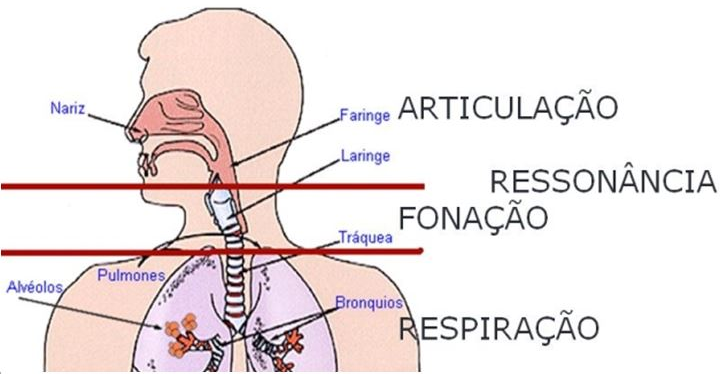
\includegraphics[width=13cm]{figuras/fisiologia-da-voz.png} %
	\label{figura:trato_vocal}
\end{figure}

%%%%%%%%%%%%%%%%%%%%%%%%%%%%%%%%%%%%%%%%%%%%%%%%%%%%%%%%
% SECAO
%%%%%%%%%%%%%%%%%%%%%%%%%%%%%%%%%%%%%%%%%%%%%%%%%%%%%%%%
\section{Sinais Digitais}
\label{sinais_digitais}
\par Os dados podem ser representados de duas maneiras: digital ou anal\'{o}gica. Sendo a primeira forma uma onda eletromagn\'{e}tica que pode assumir infinitos valores ao longo do tempo e um excelente exemplo desse tipo de sinal, \'{e} a voz humana. J\'{a} a segunda forma tem um n\'{u}mero finito de valores discretos no tempo. Em outras palavras, o sinal digital assumi valores em determinados instantes de tempo e sua representa{\c c}\~{a}o pode ser baseada na discretiza{\c c}\~{a}o de um sinal anal\'{o}gico.

\par Para se realizar uma an\'{a}lise em um sinal anal\'{o}gico em um computador, precisamos necessariamente fazer sua convers\~{a}o para a forma digital, uma vez que os computadores possuem uma capacidade finita de processamento, o que o permite tratar apenas valores discreto, n\~{a}o sendo poss\'{i}vel assim processar os infinitos pontos de um sinal anal\'{o}gico. Esse processo de convers\~{a}o \'{e} denominado de digitaliza{\c c}\~{a}o, que \'{e} realizado atrav\'{e}s das 3 etapas. Na figura 2.1 \'{e} apresentado o processo de amostragem e quantiza{\c c}\~{a}o que ser\~{a}o comentados a seguir.

\begin{enumerate}
	\item{} \textbf{Amostragem:} Consiste no processo de obter amostras de um sinal anal\'{o}gico em instantes de tempo com espa{\c c}os iguais. Vale ressaltar que para se obter sucesso nesse processo de amostragem, \'{e} necess\'{a}rio seguir o Teorema de Nyquist. Tal teorema define que para realizar a amostragem de um sinal, \'{e} necess\'{a}rio no m\'{i}nimo ter uma taxa de amostra duas vezes maior que a m\'{a}xima frequ\^{e}ncia do sinal anal\'{o}gico. Caso n\'{a}o se obtenha tal taxa de amostragem ocorrer\'{a} um efeito chamado de \textit{aliasing}, que consiste na medi{\c c}\~{a}o erronea de uma frequ\^{e}ncia mais alta como sendo mais baixa. Um bom exemplo da apli{\c c}\~{a}o de tal teorema \'{e} na digitaliza{\c c}\~{a}o da voz humana, que possui uma frequ\^{e}ncia m\'{a}xima de 4 mil Hertz. Logo, para realizar amostragem desse sinal, seria necess\'{a}rio no m\'{i}nimo 8 mil amostras por segundo.
	\item{} \textbf{Quantiza{\c c}\~{a}o:} Esse processo consiste atribui{\c c}\~{a}o de valores discretos para as amplitudes do sinal anal\'{o}gico, que pertencem a um intervalo cont\'{i}nuo de valores. Cada amplitude \'{e} alocada ao n\'{i}vel de valor discreto mais pr\'{o}ximo, o que diminui assim os erros absolutos. Vale ressalvar que o n\'{u}mero de n\'{i}veis \'{e} definido pelo n\'{u}mero de \textit{bits} que ser\~{a}o utilizados na etapa posterior de codifica{\c c}\~{a}o, que \'{e} definido como sendo ${2^n}$, onde ${n}$ \'{e} o n\'{u}mero de bits que ser\'{a} usado. De modo geral, no sinal de \'{a}udio \'{e} utilizada a quantiza{\c c}\~{a}o de 16 \textit{bits}, em outras palavras, as amplitudes de cada amostra podem assumir ${2^{16}}$  = 65536 valores. 
	
	\par Para realizar a quantiza{\c c}\~{a}o, pode-se utilizar duas t\'{e}cnicas diferentes para diminuir a quantidade de erros do processo:
	
	\begin{enumerate}
		\item {} \textbf{Quantiza{\c c}\~{a}o uniforme:} Essa t\'{e}cnica \'{e} aplicado em sinais que possuam uma pequena diferen{\c c}a entre sua amplitude m\'{a}xima e m\'{i}nima. O processo consiste em dividir de forma igualmente espa{\c c}ados os intervalos de amplitude, ou seja de forma uniforme.
		\item {} \textbf{Quantiza{\c c}\~{a}o n\~{a}o uniforme:} \'{E} utilizada para sinais que possuam um range din\^{a}mico alto, ou seja existe uma grande diferen{\c c}a entre a amplitude \'{a}xima e m\'{i}nima. Esse processo consiste em encontrar valores adequados para regi\~{a}o do sinal, o que exige diferentes quantifizadores. Um solu{\c c}\~{a}o alternativa para esse tipo de abordagem, seria comprimir o sinal, e logo ap\'{o}s utilizar a t\'{e}cnica de quantiza{\c c}\~{a}o uniforme.
	\end{enumerate}
	
	\par  Vale ressaltar que cada t\'{e}cnica descrita anteriormente depender\'{a} do sinal a ser quantificado.
	
	\item{}	\textbf{Codifica{\c c}\~{a}o:} Etapa que consiste na modifica{\c c}\~{a}o de um sinal para uma aplica{\c c}\~{a}o espec\'{i}fica, como por exemplo o armazenamento ou transmiss\~{a}o de dados.
\end{enumerate}


\begin{figure}[h]
	\centering
	\caption{(a) Sinal na forma anal\'{o}gica. (b) Amostragem. (c) Quantiza{\c c}\~{a}o, extra\'{i}do de [18]}
	
	\centering % para centralizarmos a figura
	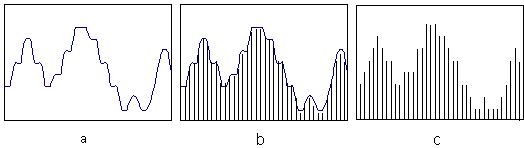
\includegraphics[width=13cm]{figuras/quant_amost.png} % leia abaixo
	\label{figura:quantizacao}
\end{figure}


%%%%%%%%%%%%%%%%%%%%%%%%%%%%%%%%%%%%%%%%%%%%%%%%%%%%%%%%
% SECAO
%%%%%%%%%%%%%%%%%%%%%%%%%%%%%%%%%%%%%%%%%%%%%%%%%%%%%%%%
\section{Arquivos Ac\'{u}sticos no Formato \textit{WAVE}}
\label{secao_formato wave}

\par\textit{Waveform audio file format} \'{e} a abrevia\c{c}\~{a}o de \textit{WAVE} ou simplesmente \textit{WAV}, que \'{e} um tipo de formato de arquivo de \'{a}udio que foi desenvolvido pela \textit{Microsoft} em conjunto com a IBM. O formato \textit{WAVE} \'{e} amplamente utilizado em uma variedade de trabalhos, sejam eles cient\'{i}ficos ou profissionais, visto que o formato permite uma fiel representa\c{c}\~{a}o dos dados digitalizados, uma vez que os dados digitalizados podem ser armazenados sem sofrer obrigatoriamente um processo de compress\~{a}o, o que evita perdas. Por\'{e}m, devido a essa caracter\'{i}stica o \textit{WAV} ocupa muito mais espa\c{c}o que os demais formatos de arquivos de \'{a}udios. 

\par Na Tabela 2.1 pode-se ver a estrutura de um arquivo \textit{WAVE}. Basicamente o arquivo \'{e} divido em 2 grandes blocos, sendo o primeiro bloco um cabe{\c c}alho RIFF e o segundo bloco \'{e} divido em dois sub-blocos, sendo um com informa{\c c}\~{o}es referentes ao formato \textit{WAVE} e o outro com os dados do \'{a}udios.

\begin{table}[h] 
	\centering
	\caption{Estrutura de um arquivo \textit{WAVE}}
	\begin{tabular}{c|c|c|c}
		\textbf{Classe} & \textbf{Posi\c{c}\~{a}o \textit{(bytes)}} & \textbf{Tamanho \textit{(bytes)}} & \textbf{Descri\c{c}\~{a}o}\\
		\hline
		Cabe\c{c}alho & 0 & 4 & Apresenta o identificador do cabe\c{c}alho - "RIFF".\\
		Cabe\c{c}alho & 4 & 4 & Tamanho do arquivo sem o identificado do cabe\c{c}alho.\\
		Cabe\c{c}alho & 8 & 4 & Mostra o identificador \textit{WAVE}.\\
		\hline
		Formato & 12 & 4 & Mostra o identificador do segundo bloco - "fmt".\\
		Formato & 16 & 4 & Tamanho do bloco sem o identificador.\\
		Formato & 20 & 2 & Mostra se o arquivo \'{e} do tipo PCM ou se tem alguma \\ & & & compress\~{a}o.\\
		Formato & 22 & 2 & Mostra a quantidade de canais.\\
		Formato & 26 & 4 & Apresenta o valor da taxa de amostragem.\\
		Formato & 30 & 4 & Apresenta a taxa de \textit{bytes}.\\
		Formato & 32 & 2 & Demostra a quantidade de \textit{bytes} para uma amostra.\\
		Formato & 34 & 2 & Demostra a quantidade de \textit{bits} para cada amostra.\\
		\hline
		Dados & 36 & 4 & Apresenta o identificador do terceiro bloco - "\textit{data}".\\
		Dados & 40 & 4 & Mostra o tamanho do bloco sem o identificador.\\
		Dados & 44 & 4 & Demostra os dados reais da m\'{u}sica.
		
	\end{tabular}
\end{table}  

\par Vale ressaltar que os valores mais comuns para cada amostra de um  arquivo \textit{WAVE} pode ser 8 \textit{bits} ou 16 \textit{bits}. Um \'{a}udio de 8 \textit{bits} siginifica que o valor da amplitude do sinal, de cada amostra, pode ser representado por 256 valores, sendo 127 positivos e 128 negativos. J\'{a} para um arquivo 16 \textit{bits} a amplitude do sinal pode ser representado por 65536 valores, com 32757 positivos e 32768 negativos. Para \textit{WAVE} de 16 \textit{bits} \'{e} utilizada a codifica{\c c}\~{a}o de complemento de 2 para representar o valor da amplitude do sinal. Assim, o valor do \textit{bit} mais significativo representa se o sinal \'{e} negaivo ou positivo.

\par Nesse trabalho foi utilizado o formato \textit{WAV} de 16 \textit{bits} PCM (\textit{Pulse-code Modulation}) que n\~{a}o utiliza compress\~{a}o, para se obter assim uma melhor qualidade na elabora\c{c}\~{a}o deste projeto final. Foi fornecida uma biblioteca escrita em C/C++ pelo orientador para isolar o primeiro bloco referente ao cabe{\c c}alho RIFF e o sub-bloco de formato \textit{WAV} dos dados brutos, que cont\'{e}m as amplitudes dos sinais de voz digitalizados.

  

%%%%%%%%%%%%%%%%%%%%%%%%%%%%%%%%%%%%%%%%%%%%%%%%%%%%%%%%
% SECAO
%%%%%%%%%%%%%%%%%%%%%%%%%%%%%%%%%%%%%%%%%%%%%%%%%%%%%%%%
\section{Reconhecimento de Padr\~{o}es e Vetores de Caracter\'{i}sticas}
\label{reconhecimento_padroes_vetores_caracteristicas}

\par Reconhecimento de Padr\~{o}es tamb\'{e}m conhecido como \textit{Pattern Recognition} ou simplesmente como PR, \'{e} uma \'{a}rea de estudo que tem como objetivo classificar objetos em determinadas classes ou categorias com base nas extra{\c c}\~{a}o de caracter\'{i}sticas relevantes de tais objetos. De modo geral, as etapas do PR pode ser dividida da seguinte maneira:

\begin{itemize}
	
	\item{
		\textbf{Extra{\c c}\~{a}o das caracter\'{i}sticas:} Principal etapa de todo o processo de \textit{Pattern Recognition}, pois \'{e} nesse momento que \'{e} realizada a redu{\c c}\~{a}o de dimensionalidade do objeto. Caso esse processo seja mal elaborado, ocorrer\'{a} perdas de caracter\'{i}sticas significativas, que podem tornar a classifica{\c c}\~{a}o dispendiosa. Portanto, \'{e} necess\'{a}rio ter um conhecimento espec\'{i}fico sobre o problema, para poder realizar a redu{\c c}\~{a}o de dimensionalidade sem que ocorr\'{a} perdas de informa{\c c}\~{o}es relevantes do objeto e tamb\'{e}m que diminua o esfor{\c c}o computacional. 
		\par Nessa etapa \'{e} realizada tamb\'{e}m a extra{\c c}\~{a}o das caracter\'{i}sticas do objeto, logo \'{e} interessante realizar uma sele{\c c}\~{a}o de modo que tais caracter\'{i}sticas sejam relevantes na classifica{\c c}\~{a}o.
	}		 
	
	\item{
		\textbf{Classifica{\c c}\~{a}o do objeto:} Etapa que determina os procedimentos para realizar a classifica{\c c}\~{a}o do objeto em um determinada classe. Diferentemente da fase anterior, o classificador pode ser definido independente do problema, uma vez que os m\'{e}todos usados s\~{a}o os mesmos .
		\par\'{E} nessa etapa que o classificador aprende a distinguir \'{a} qual classe o objeto pertencer\'{a}, de modo que esse aprendizado pode ser classificado em duas principais categorias:
		
		\begin{itemize}
			\item \textbf{Aprendizagem supervisionada:} Seu funcionamento \'{e} baseado em exemplos de entradas e sa\'{i}das previamente conhecidos, o que permite assim, aprender uma regra gen\'{e}rica para classificar as entradas posteriores. Nesse trabalho \'{e} utilizada a dist\^{a}ncia Euclidiana para tomar a decis\~{a}o de classifica{\c c}\~{a}o dos comandos falados.
			\item \textbf{Aprendizagem n\~{a}o supervisionada:} Ao contr\'{a}rio da aprendizagem supervisionada, nessa t\'{e}cnica n\~{a}o \'{e} utilizado nenhum conhecimento pr\'{e}vio para se classificar os objetos.
		\end{itemize}
}	
\end{itemize}

\par Vale ressaltar que o conceito de caracter\'{i}stica definido aqui \'{e} entendido como qualquer medida \'{u}til que possa ser extra\'{i}da no processo de identifica{\c c}\~{a}o de um padr\~{a}o. Nesse trabalho a caracter\'{i}stica escolhida para fazer a classifica{\c c}\~{a}o dos sinais foi sua energia. Ao final do processo de extra{\c c}\~{a}o todos os \'{a}udios foram convertidos em vetores de caracter\'{i}sticas com tamanhos fixos.

%%%%%%%%%%%%%%%%%%%%%%%%%%%%%%%%%%%%%%%%%%%%%%%%%%%%%%%%
% SECAO
%%%%%%%%%%%%%%%%%%%%%%%%%%%%%%%%%%%%%%%%%%%%%%%%%%%%%%%%
\section{Energia}
\label{energia}
\par A defini{\c c}\~{a}o de energia est\'{a} relacionada ao conceito de conseguir realizar trabalho. Neste projeto, ser\'{a} considerada energia a capacidade das estruturas voc\'{a}licas e dos pulm\~{o}es de produzir um sinal ac\'{u}stico. Na equa{\c c}\~{a}o 2.1 definida a energia total E(s[.]), de um dado sinal de \'{a}udio digitalizado s[.], de tamanho M.

\begin{equation}
	E(s[.])=\sum_{i = 0}^{M-1} (Si)^2
\end{equation}

\par Para realizar a captura das caracter\'{i}ticas dos \'{a}udios foi utilizado o m\'{e}todo A3, que foi referenciado pelo pr\'{o}prio orientador em \cite{Guido_tutorial}, conforme \'{e} mostrado na figura 2.3. Para realizar a extra{\c c}\~{a}o das caracter\'{i}sticas, tal m\'{e}todo se baseia no em determinar tamanhos ou \'{a}reas proporcionais para atingir n\'{i}veis predefinidos da energia do sinal que se encontra em an\'{a}lise. A3 \'{e} ideal para avaliar os n\'{i}veis de energia de um sinal de voz digitalizado que foi gerado por um agente.

\begin{figure}[h]
	\caption{[1]}
	
	\centering % para centralizarmos a figura
	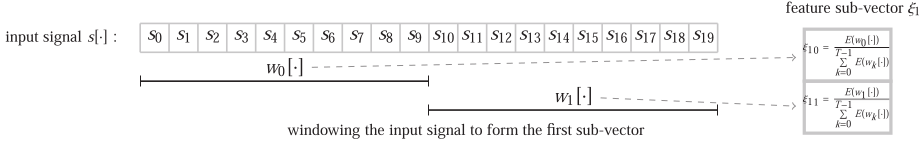
\includegraphics[width=18cm]{figuras/vetor_caracteristicas1.png}
	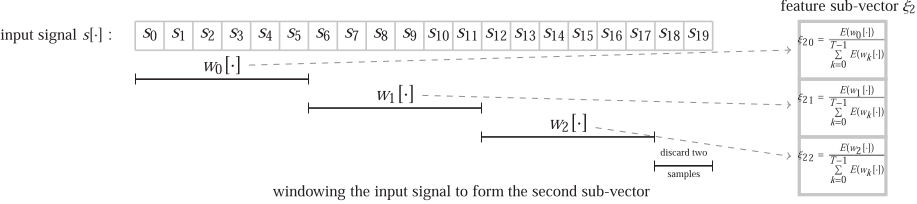
\includegraphics[width=18cm]{figuras/vetor_caracteristicas2.png}
	\label{figura:energia_vetor}
\end{figure}

\par Vale ressaltar que A3 defini um n\'{i}vel cr\'{i}tico de energia que varia de 0 a 100{\%}. Em um sinal de \'{a}udio, A3 extrai um vetor de caracter\'{i}sticas dividindo o \'{a}udio em partes proporcionais ao valor definido pelo n\'{i}vel cr\'{i}tico - par\^{a}metro C - de modo que, cria uma janela de tamanho C{\%} e extrai a caracter\'{i}stica dessa faixa de valores do sinal digitalizado, conforme \'{e} mostrado na equa{\c c}\~{a}o 2.2, onde $\epsilon$ \'{e} uma caracter\'{i}stica extraida, E(W0[.]) a energia obtida do in\'{i}cio do sinal at\'{e} o ponto final da janela definido por C, E(Wk[.]) \'{e} a energia total do sinal. Tal processo \'{e} repetido at\'{e} que se atinja o montante total de energia do \'{a}udio, de modo que, defini-se assim um vetor de caracter\'{i}sticas. 

\begin{equation}
	\epsilon = (E(W0[.]) / (\sum_{k = 0}^{T-1}E(Wk[.])))
\end{equation}  
%%%%%%%%%%%%%%%%%%%%%%%%%%%%%%%%%%%%%%%%%%%%%%%%%%%%%%%%
% SECAO
%%%%%%%%%%%%%%%%%%%%%%%%%%%%%%%%%%%%%%%%%%%%%%%%%%%%%%%%
\section{Similaridade baseada em distancias}
\label{similaridade_baseada_em_distancias}

\par Quando precisamos agrupar objetos, normalmente utilizamos como quesito a similaridade ou dissimilaridade entre tais objetos. A primeira mede o quanto dois ou mais objetos s\~{a}o parecidos entre si, enquanto que a segunda analisa o quanto dois ou mais objetos s\~{a}o diferentes.

\par Em espec\'{i}fico para avaliar similaridades em determinados objetos, podemos usufruir de uma s\'{e}rie de m\'{e}todos, sendo um dos mais conhecidos a dist\^{a}ncia Euclidiana, que pode ser calculada com base na equa{\c c}\~{a}o 2.3, onde P = $\{$P1, P2, ..., Pn$\}$ e Q = $\{$Q1, Q2, ..., Qn$\}$ s\~{a}o dois vetores de caracter\'{i}sticas e a dist\^{a}ncia d ser\'{a} o n\'{i}vel de similaridade entre os dois vetores. A similaridade entre dois objetos ser\'{a} m\'{a}xima quando P = Q, caso seja igual {\`a} zero, ser\'{a} m\'{i}nima.

\begin{equation}
	d(P, Q) = \sqrt{(P1-Q1)^2 + (P2-Q2)^2 + ... + (Pn-Qn)^2} =\sqrt{\sum_{i = 1}^{n}(Pi-Qi)^2}
\end{equation}

\vspace*{+10pt}

\par Outro m\'{e}todo para medir similaridade \'{e} atrav\'{e}s do uso da dist\^{a}ncia absoluta. Tal t\'{e}cnica utiliza o m\'{o}dulo da diferen{\c c}a entre dois n\'{u}meros para realizar a medi{\c c}\~{a}o, conforme \'{e} mostrado na equa{\c c}\~{a}o 2.4. Caso a diferen{\c c}a seja igual a zero, temos que os dois objetos comparados s\~{a}o identicos, caso contr\'{a}rio, ser\~{a}o diferentes.

\begin{equation}
	d = |X - Y|
\end{equation}

\par O classificador que \'{e} elaborado nesse presente trabalho, foi implementado com o m\'{e}todo de dist\^{a}ncia Euclidiana, visto que tal m\'{e}trica oferece al\'{e}m de simplificade, \'{o}timos resultados para reconhecimento de padr\~{o}es em sinais ac\'{u}sticos \cite{Marcel_Kfouri}.

%%%%%%%%%%%%%%%%%%%%%%%%%%%%%%%%%%%%%%%%%%%%%%%%%%%%%%%%
% SECAO
%%%%%%%%%%%%%%%%%%%%%%%%%%%%%%%%%%%%%%%%%%%%%%%%%%%%%%%%
\section{Trabalhos Correlatos}
\label{trabalhos_correlatos}
\par A \'{a}rea de \textit{speech recognition} tem sido bastante estudada em diversas trabalhos. Nas monografias de conclus\~{a}o de curso [2, 4, 5, 6, 12, 13, 14] \'{e} discutido temas sobre o reconhecimento de vacabul\'{a}rio restrito. J\'{a} nos artigos [15, 16] os esfor{\c c}os s\~{a}o voltados para o reconhecimento de um amplo vocabul\'{a}rio, tal como idiomas.

\par Em [2], o autor utiliza conceitos como energia, limiar \textit{hard}, n\'{i}veis cr\'{i}ticos de energia, para elaborar um sistema  de reconhecimento de vocabul\'{a}rio restrito implementado na linguagem C/C++, com um classificador baseado em dist\^{a}ncia Euclidiana.

\par Em [4], o autor utiliza duas abordagens diferentes para realizar o reconhecimento de voz, sendo a primeira baseada em \textit{pattern-matching} e a outra em \textit{knowledge-based}. Ao final do trabalho pode-se concluir e verificar que a segunda abordagem apresentou melhores resultados, pois utilizava intelig\^{e}ncia artificial.

\par Particularmente em [5], o autor prop\~{o}em um sistema para reconhecimento de voz independente do locutor. Para isso, o autor utiliza conceitos como  \textit{Zero Crossing Rate} e energia para realizar o pr\'{e}-processamento, extra{\c c}\~{a}o de caracter\'{i}sticas e um classificador tamb\'{e}m baseado em dist\^{a}ncia Euclidiana.

\par Em [7], o autor desenvolve um sistema de reconhecimento de voz baseado em automa{\c c}\~{a}o residencial via wireless. Para a elabora{\c c}\~{a}o desse projeto, o autor utiliza o dispositivo HM2007L IC, para assim realizar o reconheicmento de comandos simples, como "acender", "apagar", acender a luz", etc.

\par Em [8], o objetivo do autor \'{e} melhorar a rela{\c c}\~{a}o homem-m\'{a}quina, e com isso, desenvolve um m\'{e}todo para reconhecimento de voz que uso de caracter\'{i}sticas \textit{voice-likeness}.

\par Em [9] o autor tem como objetivo desenvolver um sistema para \textit{smartphone} multifuncional que al\'{e}m de realizar o reconhecimento de voz, tamb\'{e}m a fa{\c c}a a convers\~{a}o do di\'{a}logo reconhecido para texto.

\par Em [13], o autor utiliza conceitos como MFCC, HMM (\textit{Hidden Markov Models}), para reconhecer um restrito vocabul\'{a}rio que contem digitos de 0 a 9.

\par J\'{a} em [16], \'{e} realizada uma compara{\c c}\~{a}o de desempenho de GMMs - Modelos de Misturas Gaussianas - com DNNs - Redes Neurais Profundas - no reconhecimento de um amplo vocabul\'{a}rio Chines. 

\par Em [17], com o objetivo de melhorar a efic\'{a}cia do reconhecimento de um vocabul\'{a}rio Russo amplo, foi utilizado t\'{e}cnicas \textit{knowledge-based} e estat\'{i}sticas para modelagem de fonemas.



%%%%%%%%%%%%%%%%%%%%%%%%%%%%%%%%%%%%%%%%%%%%%%%%%%%%%%%%
% CAPITULO 3
%%%%%%%%%%%%%%%%%%%%%%%%%%%%%%%%%%%%%%%%%%%%%%%%%%%%%%%%
%%%%%%%%%%%%%%%%%%%%%%%%%%%%%%%%%%%%%%%%%%%%%%%%%%%%%%%%
\chapter{Detalhamento do Trabalho Proposto}
\label{cap3}
\thispagestyle{myheadings}
%%%%%%%%%%%%%%%%%%%%%%%%%%%%%%%%%%%%%%%%%%%%%%%%%%%%%%%%
% SECAO
%%%%%%%%%%%%%%%%%%%%%%%%%%%%%%%%%%%%%%%%%%%%%%%%%%%%%%%%
\vspace*{-0.3cm}
\section{Estrutura do Sistema}
\label{estrutura_sistema}

%%%%%%%%%%%%%%%%%%%%%%%%%%%%%%%%%%%%%%%%%%%%%%%%%%%%%%%%
% SECAO
%%%%%%%%%%%%%%%%%%%%%%%%%%%%%%%%%%%%%%%%%%%%%%%%%%%%%%%%
\section{Coleta e elabora{\c c}\~{a}o do banco de \'{a}udios}
\par Inicialmente, foram definidos os 11 comandos que ser\~{a}o reconhecidos pelo sistema, conforme j\'{a} mencionado. Os comandos foram gravados 10 vezes em diferentes dias e hor\'{a}rios, para obter se assim, uma melhor veracidade e fidelidade \`{a} voz do locutor, pois o mesmo pode sofrer altera{\c c}\~{o}es significativas com base na varia{\c c}\~{a}o do seu humor ou estado f\'{i}sico. Como tamb\'{e}m j\'{a} mencionado, a grava{\c c}\~{a}o dos arquivos de \'{a}udio foi realizada em um ambiente fechado, para diminuir assim, a probabilidade de ru\'{i}dos nos sinais. Todos os arquivos foram gravados no formato MPEG-4, que \'{e} o formato dispon\'{i}vel no \textit{software} de grava{\c c}\~{a}o de \'{a}udio do \textit{Windows} 10, e posteriormente foram convertidos para o formato \textit{WAVE} de 16 \textit{bits} PCM, com o aux\'{i}lio do editor de \'{a}udio \textit{Audacity}. Ao total, foram gravados e convertidos 110 arquivos de \'{a}udio.
%%%%%%%%%%%%%%%%%%%%%%%%%%%%%%%%%%%%%%%%%%%%%%%%%%%%%%%%
%%%%%%%%%%%%%%%%%%%%%%%%%%%%%%%%%%%%%%%%%%%%%%%%%%%%%%%%
% CAPITULO 4
%%%%%%%%%%%%%%%%%%%%%%%%%%%%%%%%%%%%%%%%%%%%%%%%%%%%%%%%
%%%%%%%%%%%%%%%%%%%%%%%%%%%%%%%%%%%%%%%%%%%%%%%%%%%%%%%%
\chapter{Testes e Resultados}
\label{cap4}
\thispagestyle{myheadings}
bla bla bla...
%%%%%%%%%%%%%%%%%%%%%%%%%%%%%%%%%%%%%%%%%%%%%%%%%%%%%%%%
%%%%%%%%%%%%%%%%%%%%%%%%%%%%%%%%%%%%%%%%%%%%%%%%%%%%%%%%
% CAPITULO 5
%%%%%%%%%%%%%%%%%%%%%%%%%%%%%%%%%%%%%%%%%%%%%%%%%%%%%%%%
%%%%%%%%%%%%%%%%%%%%%%%%%%%%%%%%%%%%%%%%%%%%%%%%%%%%%%%%
\chapter{Conclus\~{o}es e Trabalhos Futuros}
\label{cap5}
\thispagestyle{myheadings}
\par Neste trabalho, ...
%%%%%%%%%%%%%%%%%%%%%%%%%%%%%%%%%%%%%%%%%%%%%%%%%%%%%%%%
%%%%%%%%%%%%%%%%%%%%%%%%%%%%%%%%%%%%%%%%%%%%%%%%%%%%%%%%
% REFERENCIAS
%%%%%%%%%%%%%%%%%%%%%%%%%%%%%%%%%%%%%%%%%%%%%%%%%%%%%%%%
%%%%%%%%%%%%%%%%%%%%%%%%%%%%%%%%%%%%%%%%%%%%%%%%%%%%%%%%
\renewcommand
\bibname{\centering{Refer\^{e}ncias}}
\addcontentsline{toc}{chapter}{Refer\^{e}ncias}
\begin{thebibliography}{00}
\thispagestyle{myheadings}
\bibliographystyle{abnt-num}

\bibitem{Guido_tutorial}
	\begin{singlespace}
		GUIDO, R. C. A tutorial on signal energy and its applications. Neurocomputting, v. 179, p.264-282, 2016.
	\end{singlespace}


\bibitem{Marcel_Kfouri}
\begin{singlespace}
	DORDAN, M, K. Verifica{\c c}\~{a}o de Locutores dependente do discurso baseada na Evolu{\c c}\~{a}o do Esfor{\c c}o Voc\'{a}lico. IBILCE, UNESP, S\~{a}o Jos\'{e} do Rio Preto (Trabalho de Conclus\~{a}o de Gradua{\c c}\~{a}o em Ci\~{e}ncia da Computa{\c c}\~{a}o), 2015.
\end{singlespace}

\bibitem{Vinicius_Francisco}
\begin{singlespace}
	SILVA, V. F. Identifica{\c c}\~{a}o e Classifica{\c c}\~{a}o de G\~{e}neros Musicais com Abordagens M\'{u}ltiplas de Reconhecimento de Padr\~{o}es. IBILCE, UNESP, S\~{a}o Jos\'{e} do Rio Preto (Trabalho de Conclus\~{a}o de Gradua{\c c}\~{a}o em Ci\~{e}ncia da Computa{\c c}\~{a}o), 2014.
\end{singlespace}


\bibitem{Ana_Paula}
\begin{singlespace}
	CAOBIANCO, A. P. Compara{\c c}\~{a}o de Abordagens \textit{PatternMatching} e \textit{Knowledge-Based} para Reconhecimento de Locutor Dependente de Texto. IBILCE, UNESP, S\~{a}o Jos\'{e} do Rio Preto (Trabalho de Conclus\~{a}o de Gradua{\c c}\~{a}o em Ci\~{e}ncia da Computa{\c c}\~{a}o), 2011.
\end{singlespace}

\bibitem{João_Vitor_Maschio}
\begin{singlespace}
	MASCHIO, J. V. D. Projeto e Implementa{\c c}\~{a}o Ac\'{u}stico-Computacional de Palavras Isoladas. IBILCE, UNESP, S\~{a}o Jos\'{e} do Rio Preto (Trabalho de Conclus\~{a}o de Gradua{\c c}\~{a}o em Ci\~{e}ncia da Computa{\c c}\~{a}o), 2017.
\end{singlespace}

\bibitem{Reconhecimento_Comandos_Falados_Portugues_Brasileiro}
\begin{singlespace}
	LOUREIRO, W. d. F. Reconhecimento de Comandos Falados Portugu\^{e}s Brasileiro com Par\^{a}metros de Frequ\^{e}ncia e Tempo. IBILCE, UNESP, S\~{a}o Jos\'{e} do Rio Preto (Trabalho de Conclus\~{a}o de Gradua{\c c}\~{a}o em Ci\~{e}ncia da Computa{\c c}\~{a}o), 2015.
\end{singlespace}

\bibitem{Voice_recognition_Room_automation}
\begin{singlespace}
	PAUL, A.; PANJA, M.; BAGCHI, M.; DAS, N.; MAZUMDER, R. M.; GHOSH, S. Voice Recognition Based Wireless Room Automation
	System. 2016 International Conference on Intelligent Control Power and Instrumentation, 2016.
\end{singlespace}

\bibitem{Laughing_Voice_Recognition}
\begin{singlespace}
	SAKANO, T.; KIGAWA, T.; SUGIMOTO, M.; KUSUNOKI, F.; INAGAKI, F.; MIZOGUCHI, H. Laughing Voice Recognition Using Periodic Waveforms and Voice-likeness Features. Proceedings of the 2016 IEEE International Conference on Robotics and Biomimetics Qingdao, China, 2016.
\end{singlespace}

\bibitem{A_Smartphone-Based_Multi-Functional_Hearing}
\begin{singlespace}
	CHERN, A.; TSAO, Y.; CHANG, R.; HSIU-WEN, C.; YING-HUI, L. A Smartphone-Based Multi-Functional Hearing Assistive System to Facilitate Speech Recognition in the Classroom. Dispon\'{i}vel em: $<$http://ieeexplore.ieee.org/document/7938619/$>$. Acesso em: 05 jun. 2017.
\end{singlespace}

\bibitem{Fundamentals_of_speech_recognition}
\begin{singlespace}
	RABINER, L. R; JUANG, B. H. Fundamentals of Speech Recognition. Prentice Hall, 1993.
\end{singlespace}

\bibitem{Pattern Classification}
\begin{singlespace}
	DUDA, R. O.; HART, P. E.; STORK, D. G. Pattern Classification. 2. ed. Wiley-Interscience, 2000.
\end{singlespace}

\bibitem{Pattern Recognition}
\begin{singlespace}
	THEODORIDIS, S.; KOUTROUMBAS, K. Pattern Recognition. 4. ed, Academic Press, 2008.
\end{singlespace}

\bibitem{Reconhecimento_voz_palavras_isoladas}
\begin{singlespace}
	SILVA, A. G. d. Reconhecimento de Voz para Palavras Isoladas. Monografia (Gradua{\c c}\~{a}o em Engenharia da Computa{\c c}\~{a}o) - UFPE, Recife, 2009.
\end{singlespace}

\bibitem{Reconhecimento_automatico_fala_computador}
\begin{singlespace}
	LOUZADA, J. Reconhecimento Autom\'{a}tico de Fala por Computador. Monografia(Gradua{\c c}\~{a}o em Ci\~{e}ncia da Computa{\c c}\~{a}o) - PUC, Goi\'{a}s, 2010.
\end{singlespace}

\bibitem{Reconhecimento_padrao_formato_wave}
\begin{singlespace}
Piccoli, E. E. M. Reconhecimento de Padr\~{a}o em \'{A}udio no Formato Wave. IBILCE, UNESP, S\~{a}o Jos\'{e} do Rio Preto (Trabalho de Conclus\~{a}o de Gradua{\c c}\~{a}o em Ci\~{e}ncia da Computa{\c c}\~{a}o), 2014.
\end{singlespace}

\bibitem{reconhecimento_vocabulario_chines}
\begin{singlespace}
	LI, X.; YANG, Y.; PANG, Z.; WU, X. A Comparative Study on Selecting Acoustic Modeling Units in Deep Neural Networks Based large Vocabulary Chinese Speech Recognition. Neurocomputing, v. 170, p. 251-256, 2015
\end{singlespace}

\bibitem{Reconhecimento_vocabulario_russo}
\begin{singlespace}
	KARPOV, A.; MARKOV, K.; KIPYATKOVA, I.; VAZHENINA, D.; RONZHIN, A.; Large Vocabulary Russian Speech Recognition Using Syntactico-statistical language Modeling. Speech Communication, v.56, p.213-228, 2014.
\end{singlespace}

\bibitem{imagem_quantizacao}
\begin{singlespace}
	Figura extra\'{i}da de: $<$http://penta3.ufrgs.br/RNP/cap3/3.2%20Audio/$>$. Acesso em: 20 Abril 2017. 
\end{singlespace}

\bibitem{voz}
\begin{singlespace}
	Figura extra\'{i}da de: $<$http://www.koreapost.com.br/wp-content/uploads/2016/01/fisiologia-da-voz.jpg$>$. Acesso em: 18 Abril 2017. 
\end{singlespace}



\end{thebibliography}
%%%%%%%%%%%%%%%%%%%%%%%%%%%%%%%%%%%%%%%%%%%%%%%%%%%%%%%%
%%%%%%%%%%%%%%%%%%%%%%%%%%%%%%%%%%%%%%%%%%%%%%%%%%%%%%%%
% APENDICE
%%%%%%%%%%%%%%%%%%%%%%%%%%%%%%%%%%%%%%%%%%%%%%%%%%%%%%%%
%%%%%%%%%%%%%%%%%%%%%%%%%%%%%%%%%%%%%%%%%%%%%%%%%%%%%%%%
\thispagestyle{myheadings}
\newpage\ \thispagestyle{myheadings} \newpage
\thispagestyle{myheadings}

\appendix

\renewcommand{\chaptername}{Ap\^{e}ndice I - Gr\'{a}ficos das caracter\'{i}sticas extra\'{i}das}

\addcontentsline{toc}{chapter}{Ap\^{e}ndice I - Gr\'{a}ficos das caracter\'{i}sticas extra\'{i}das}

\noindent

{\huge \vspace*{+79pt} \textbf{Ap\^{e}ndice I - Gr\'{a}ficos das caracter\'{i}sticas}}
{\huge \hspace*{+11pt} \textbf{extra\'{i}das}}

\end{document}